\documentclass[11pt,openany,a4paper]{article}
\usepackage{amsmath, amsfonts, amssymb, amsthm}
\usepackage{tikz, pgfplots, tkz-euclide,calc}
    \usetikzlibrary{patterns,snakes,shapes.arrows}
\usepackage{fancyhdr}
\usepackage{enumerate,enumitem}
\usepackage{cancel}
\usepackage{varwidth}
\usepackage{hyperref}
\hypersetup{
    colorlinks=true,
    linkcolor=blue,
    filecolor=magenta,      
    urlcolor=cyan,
    }

% TAMBAHKAN PACKAGE SENDIRI KALAU KURANG

\usepackage{geometry}
\geometry{
	total = {160mm, 230mm},
	left = 16mm,
	right = 16mm,
	top = 30mm,
	bottom = 30mm,
}


\pagestyle{fancy}
\fancyhead{}
\fancyfoot{}
\fancyhead[r]{}
\fancyhead[l]{\fbox{\large{\textbf{SKPB - ITS}}}}
\renewcommand{\headrulewidth}{0pt}
\renewcommand{\footrulewidth}{0pt}


\begin{document}

\begin{center}
  {\underline{\textbf{\MakeUppercase{Tes Seleksi Asisten Dosen Semester Gasal 2026/2027}}}}
\end{center}

\begin{center}
  \begin{tabular}{lcl}
    Mata kuliah/SKS & : & Kalkulus 1 ( SM23 4 101 ) / 3 SKS \\
    Hari, Tanggal   & : & Senin, 24 Agustus 2026            \\
    Waktu           & : & 09.10-10.30 WIB (80 menit)        \\
    Sifat           & : & Tertutup
  \end{tabular}
\end{center}

\noindent\rule{\textwidth}{2.pt}

% SOAL DI SINI YAA
\begin{enumerate}
  \item \textbf{[20 POIN]} Tentukan himpunan penyelesaian dari pertidaksamaan berikut:
        \[
          |x^2 - 4| \le x + 2.
        \]

  \item \textbf{[25 POIN]} Diberikan \( f(x) = \frac{2x-1}{x+2} \) dan \( g(x) = \sqrt{x - 1} \).
        \begin{enumerate}
          \item Dapatkan domain fungsi \( f(x) \) dan \( g(x) \).
          \item Dapatkan fungsi \( f \circ f, g \circ g, f \circ g \), dan \( g \circ f \) beserta domain masing-masing.
        \end{enumerate}

  \item \textbf{[30 POIN]} Sebuah poster berbentuk persegi panjang memiliki luas \( 360 \text{ cm}^2 \). Pada poster tersebut
        terdapat daerah berbentuk persegi panjang untuk menempatkan gambar. Daerah ini berjarak \( 4 \text{ cm} \)
        dari sisi kiri dan kanan serta \( 6 \text{ cm} \) dari sisi atas dan bawah poster. Untuk menjaga proporsi desain,
        lebar daerah gambar setidaknya dua kali tinggi daerah gambar. Tentukan luas daerah gambar agar
        luasnya maksimum.

        \begin{center}
          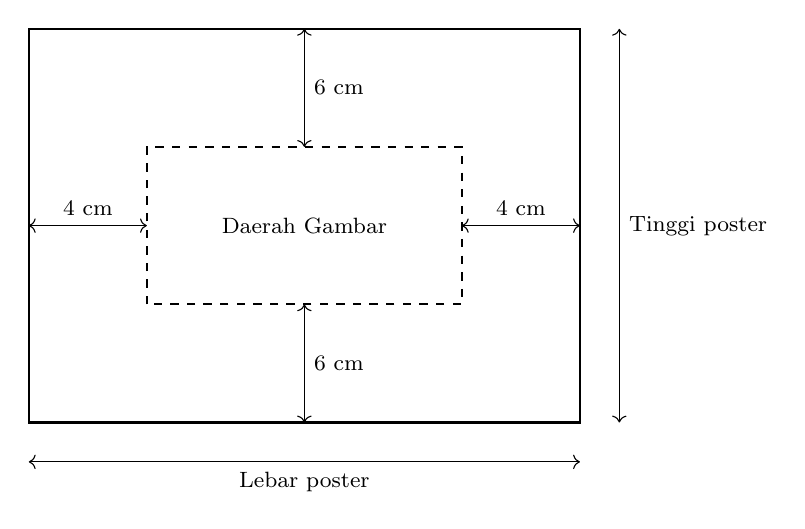
\begin{tikzpicture}
            % Outer poster
            \draw[thick] (0,0) rectangle (7,5);

            % Inner image area
            \draw[thick, dashed] (1.5,1.5) rectangle (5.5,3.5);

            % Labels
            \node at (3.5, 2.5) {\footnotesize Daerah Gambar};

            % Arrows for margins
            \draw[<->] (0, 2.5) -- (1.5, 2.5) node[midway, above] {\footnotesize 4 cm};
            \draw[<->] (5.5, 2.5) -- (7, 2.5) node[midway, above] {\footnotesize 4 cm};
            \draw[<->] (3.5, 0) -- (3.5, 1.5) node[midway, right] {\footnotesize 6 cm};
            \draw[<->] (3.5, 3.5) -- (3.5, 5) node[midway, right] {\footnotesize 6 cm};

            % External dimensions
            \draw[<->] (0, -0.5) -- (7, -0.5) node[midway, below] {\footnotesize Lebar poster};
            \draw[<->] (7.5, 0) -- (7.5, 5) node[midway, right] {\footnotesize Tinggi poster};
          \end{tikzpicture}
        \end{center}

  \item \textbf{[25 POIN]} Tentukan nilai dari
        \[
          \int_{-3}^{3} \frac{x^3 - 16}{|x| + 3} \, dx.
        \]
\end{enumerate}

%   \vspace*{2cm}
%   \hrulefill\textbf{ Selamat Mengerjakan }\hrulefill

%   \begin{center}
% "\textit{Jujur adalah kunci kesuksesan}"
%   \end{center}

\newpage
\fancyhead[L]{\textit{Solution By: \hyperlink{https://github.com/TetewHeroez}{Tetew}}}

\begin{center}
  {\underline{\textbf{\MakeUppercase{Pembahasan}}}}
\end{center}

\begin{enumerate}
  \item \textbf{Pembahasan Soal 1:} \\
        Diberikan pertidaksamaan $|x^2 - 4| \le x + 2$. \\
        Ingat kembali sifat nilai mutlak: $|A| \le B \iff -B \le A \le B$ dengan syarat $B \ge 0$. \\
        Karena ruas kiri adalah nilai mutlak (selalu bernilai non-negatif), maka ruas kanan haruslah $x + 2 \ge 0 \implies x \ge -2$. \\
        Berdasarkan sifat tersebut, diperoleh:
        \[
          -(x + 2) \le x^2 - 4 \le x + 2
        \]
        Pertidaksamaan ini dapat dipecah menjadi dua bagian yang harus dipenuhi secara bersamaan:
        \begin{enumerate}[label=(\roman*)]
          \item $-(x + 2) \le x^2 - 4$ \\
                $-x - 2 \le x^2 - 4 \implies x^2 + x - 2 \ge 0 \implies (x+2)(x-1) \ge 0$. \\
                Pembuat nol adalah $x = -2$ dan $x = 1$. Penyelesaiannya adalah $x \le -2$ atau $x \ge 1$.
          \item $x^2 - 4 \le x + 2$ \\
                $x^2 - x - 6 \le 0 \implies (x-3)(x+2) \le 0$. \\
                Pembuat nol adalah $x = 3$ dan $x = -2$. Penyelesaiannya adalah $-2 \le x \le 3$.
        \end{enumerate}
        Himpunan penyelesaian akhirnya adalah irisan dari (i) dan (ii):
        \[
          (-\infty, -2] \cup [1, \infty)  \cap  [-2, 3] = \{-2\} \cup [1, 3]
        \]
        Jadi, himpunan penyelesaiannya adalah $x = -2$ atau $1 \le x \le 3$.

  \item \textbf{Pembahasan Soal 2:}
        \begin{enumerate}
          \item Domain $f(x)$ dan $g(x)$: \\
                Fungsi $f(x) = \frac{2x-1}{x+2}$ terdefinisi jika penyebutnya tidak nol: $x + 2 \ne 0 \implies x \ne -2$. \\
                Jadi, $D_f = \{x \in \mathbb{R} \mid x \ne -2\} = \mathbb{R} \setminus \{-2\}$. \\
                Fungsi $g(x) = \sqrt{x-1}$ terdefinisi jika fungsi di dalam akar non-negatif: $x - 1 \ge 0 \implies x \ge 1$. \\
                Jadi, $D_g = \{x \in \mathbb{R} \mid x \ge 1\} = [1, \infty)$.
          \item Fungsi komposisi dan domain masing-masing:
                \begin{itemize}
                  \item $f \circ f$: \\
                        $(f \circ f)(x) = f(f(x)) = \frac{2\left(\frac{2x-1}{x+2}\right)-1}{\left(\frac{2x-1}{x+2}\right)+2} = \frac{\frac{4x-2-x-2}{x+2}}{\frac{2x-1+2x+4}{x+2}} = \frac{3x-4}{4x+3}$. \\
                        Domain $f \circ f$: $x \in D_f \land f(x) \in D_f$. \\
                        $x \ne -2 \land \frac{2x-1}{x+2} \ne -2 \implies 2x - 1 \ne -2x - 4 \implies 4x \ne -3 \implies x \ne -\frac{3}{4}$. \\
                        $D_{f \circ f} = \mathbb{R} \setminus \{-2, -\frac{3}{4}\}$.

                  \item $g \circ g$: \\
                        $(g \circ g)(x) = g(g(x)) = \sqrt{\sqrt{x-1} - 1}$. \\
                        Domain $g \circ g$: $x \in D_g \land g(x) \in D_g$. \\
                        $x \ge 1 \land \sqrt{x-1} \ge 1 \implies x - 1 \ge 1 \implies x \ge 2$. \\
                        $D_{g \circ g} = [2, \infty)$.

                  \item $f \circ g$: \\
                        $(f \circ g)(x) = f(g(x)) = \frac{2\sqrt{x-1}-1}{\sqrt{x-1}+2}$. \\
                        Domain $f \circ g$: $x \in D_g \land g(x) \in D_f$. \\
                        $x \ge 1 \land \sqrt{x-1} \ne -2$. (Karena $\sqrt{x-1} \ge 0$, maka $\sqrt{x-1} \ne -2$ dipenuhi untuk semua $x \ge 1$). \\
                        $D_{f \circ g} = [1, \infty)$.

                  \item $g \circ f$: \\
                        $(g \circ f)(x) = g(f(x)) = \sqrt{\frac{2x-1}{x+2} - 1} = \sqrt{\frac{x-3}{x+2}}$. \\
                        Domain $g \circ f$: $x \in D_f \land f(x) \in D_g$. \\
                        $x \ne -2 \land \frac{2x-1}{x+2} \ge 1 \implies \frac{x-3}{x+2} \ge 0$. \\
                        Pembuat nol pembilang dan penyebut adalah $x = 3$ dan $x = -2$. \\
                        Melalui uji garis bilangan, penyelesaiannya adalah $x < -2$ atau $x \ge 3$. \\
                        $D_{g \circ f} = (-\infty, -2) \cup [3, \infty)$.
                \end{itemize}
        \end{enumerate}

  \item \textbf{Pembahasan Soal 3:} \\
        Misalkan dimensi poster adalah lebar $x$ cm dan tinggi $y$ cm. \\
        Luas poster adalah $xy = 360 \implies y = \frac{360}{x}$. \\
        Misalkan dimensi gambar adalah lebar $l_g$ dan tinggi $t_g$.
        Sesuai dengan margin poster: \\
        $l_g = x - 4 - 4 = x - 8$ \\
        $t_g = y - 6 - 6 = y - 12 = \frac{360}{x} - 12$

        Terdapat syarat proporsi desain, yaitu lebar gambar setidaknya dua kali tinggi gambar:
        \begin{align*}
          l_g                    & \ge 2t_g                                \\
          x - 8                  & \ge 2 \left( \frac{360}{x} - 12 \right) \\
          x - 8                  & \ge \frac{720}{x} - 24                  \\
          x + 16 - \frac{720}{x} & \ge 0
        \end{align*}
        Karena $x > 0$ (lebar bernilai positif), kalikan dengan $x$:
        \[
          x^2 + 16x - 720 \ge 0 \implies (x - 20)(x + 36) \ge 0
        \]
        Karena $x > 0$, maka $x \ge 20$. \\
        Di sisi lain, dimensi gambar harus positif ($t_g > 0 \implies \frac{360}{x} > 12 \implies x < 30$). \\
        Domain untuk lebar poster adalah $20 \le x < 30$.

        Luas daerah gambar $L(x)$ dirumuskan sebagai:
        \[
          L(x) = l_g \cdot t_g = (x - 8) \left( \frac{360}{x} - 12 \right) = 360 - 12x - \frac{2880}{x} + 96 = 456 - 12x - 2880x^{-1}
        \]
        Untuk mencari luas maksimum, cari nilai kritis dengan menggunakan turunan pertama $L'(x)$:
        \[
          L'(x) = -12 + 2880x^{-2} = \frac{2880}{x^2} - 12
        \]
        Untuk menemukan titik stasioner, kita mengatur $L'(x) = 0$:
        \[
          \frac{2880}{x^2} = 12 \implies x^2 = \frac{2880}{12} = 240 \implies x = \sqrt{240} = 4\sqrt{15} \approx 15.49
        \]
        Titik kritis $x \approx 15.49$ berada di luar domain $20 \le x < 30$. \\
        Untuk interval $x \ge 20$, nilai $x^2 \ge 400$, sehingga $\frac{2880}{x^2} \le 7.2$. \\
        Karena itu, $L'(x) = \frac{2880}{x^2} - 12 \le 7.2 - 12 = -4.8 < 0$ untuk setiap $x \in [20, 30)$. \\
        Karena turunan pertamanya negatif ($L'(x) < 0$), fungsi $L(x)$ monoton turun pada interval $20 \le x < 30$. \\
        Karena fungsi monoton turun, nilai maksimum fungsi pada interval dicapai pada batas sekecil-kecilnya dari interval, yaitu di $x = 20$. \\
        Saat $x = 20$, luas daerah gambar maksimum adalah:
        \[
          L(20) = 456 - 12(20) - \frac{2880}{20} = 456 - 240 - 144 = 72 \text{ cm}^2
        \]
        Jadi, luas daerah gambar agar luasnya maksimum adalah $72 \text{ cm}^2$.

  \item \textbf{Pembahasan Soal 4:} \\
        Integral $\int_{-3}^{3} \frac{x^3 - 16}{|x| + 3} \, dx$ dapat dipisah menjadi dua integral agar dapat memanfaatkan sifat fungsi ganjil dan genap:
        \[
          \int_{-3}^{3} \frac{x^3 - 16}{|x| + 3} \, dx = \int_{-3}^{3} \frac{x^3}{|x| + 3} \, dx - \int_{-3}^{3} \frac{16}{|x| + 3} \, dx
        \]

        Tinjau integral bagian pertama:
        Misalkan $h(x) = \frac{x^3}{|x| + 3}$.
        \[
          h(-x) = \frac{(-x)^3}{|-x| + 3} = \frac{-x^3}{|x| + 3} = -h(x)
        \]
        Karena $h(-x) = -h(x)$, maka $h(x)$ adalah fungsi ganjil. Pada batas integrasi simetris $[-3, 3]$, nilai integral dari fungsi ganjil adalah $0$.
        \[
          \int_{-3}^{3} \frac{x^3}{|x| + 3} \, dx = 0
        \]

        Tinjau integral bagian kedua:
        Misalkan $p(x) = \frac{16}{|x| + 3}$.
        \[
          p(-x) = \frac{16}{|-x| + 3} = \frac{16}{|x| + 3} = p(x)
        \]
        Karena $p(-x) = p(x)$, maka $p(x)$ adalah fungsi genap. Nilai integral pada rentang $[-3, 3]$ adalah dua kali nilai integral pada rentang $[0, 3]$. Pada interval $[0, 3]$, karena $x \ge 0$, maka $|x| = x$.
        \[
          \int_{-3}^{3} \frac{16}{|x| + 3} \, dx = 2 \int_{0}^{3} \frac{16}{x + 3} \, dx = 32 \int_{0}^{3} \frac{1}{x + 3} \, dx
        \]
        Menghitung nilai integral tersebut:
        \[
          32 \int_{0}^{3} \frac{1}{x + 3} \, dx = 32 \left[ \ln|x + 3| \right]_{0}^{3} = 32 (\ln 6 - \ln 3) = 32 \ln \left(\frac{6}{3}\right) = 32 \ln 2
        \]

        Maka, nilai integral akhir adalah gabungan keduanya:
        \[
          \int_{-3}^{3} \frac{x^3 - 16}{|x| + 3} \, dx = 0 - 32 \ln 2 = -32 \ln 2
        \]
\end{enumerate}

\end{document}